\documentclass{template}

\title{MA 580 Assignment 1}
\author{Kyle Hansen}
\date{5 September 2025}

\usepackage{cancel}

\newcommand{\maxmag}{\mathrm{\mathbf{maxmag}}}
\newcommand{\minmag}{\mathrm{\mathbf{minmag}}}

\begin{document}

\maketitle

\textbf{AI Use Statement: }Here is where I put the AI use statemet

\section{}

Let $\mat{A} \in \R^{m \times n}$. 
Prove the following. 
In your solution 
use only the materials discussed in the lectures so far and results 
from the previous homework.

\subsection{}
Show that $\lambda \neq 0$ is an eigenvalue of $\mat{A}^T \mat{A}$ if and 
only if it is an eigenvalue of $\mat{A}\mat{A}^T$.

The nozero eigenvalues of $\mat{A}^T \mat{A}$ are defined such that, for some $x \neq 0$,

\begin{equation}
    (\mat{A}^T \mat{A})x = \lambda x
\end{equation}

then it can be shown that this value $\lambda$ is also an eigenvalue of $\mat{A}\mat{A}^T $:

\begin{equation}
    \begin{aligned}
    \mat{A}^T \mat{A}x &= \lambda x\\
    \mat{A}\mat{A}^T \mat{A}x &= \lambda \mat{A} x\\
    \end{aligned}
\end{equation}

Then, for some $b = \mat{A}x$, 

\begin{equation}
    (\mat{A}\mat{A}^T )b = \lambda b
\end{equation}

That is, all nonzero eigenvalues of $\mat{A}^T \mat{A}$ are also eigenvalues of $\mat{A}\mat{A}^T$.

The inverse can be shown similarly:

\begin{equation}
    \begin{aligned}
    \mat{A}\mat{A}^T x &= \lambda x\\
    \mat{A}^T \mat{A}\mat{A}^Tx &= \lambda \mat{A}^T x\\
    \end{aligned}
\end{equation}

Then for some $z=\mat{A}^Tx$, $\mat{A}^T \mat{A}z = \lambda z$. Then the matrices $\mat{A}\mat{A}^T$ and $\mat{A}^T \mat{A}$ share all non-zero eigenvalues.


\subsection{}
Show $\norm{\mat{A}^T}_2 = \norm{\mat{A}}_2$. 

This can be shown using the spectral radius, since $\norm{\mat{A}}_2 = \rho(\mat{A}^T \mat{A})^{1/2}$, which implies $\norm{\mat{A}^T}_2 = \rho(\mat{A} \mat{A}^T)^{1/2}$.

Since $\mat{A} \mat{A}^T$ and $\mat{A}^T \mat{A}$ have the same nonzero eigenvalues, then they share the same spectral radius $\rho(\mat{A}) = \text{max}|\lambda|$. Then:

\begin{equation}\label{eq:spectral-radii}
    \begin{aligned}
        \rho(\mat{A}^T \mat{A})^{1/2} &= \rho(\mat{A} \mat{A}^T)^{1/2}\\
        \norm{\mat{A}}_2 & = \norm{\mat{A}^T}_2.
    \end{aligned}
\end{equation}




\subsection{}

Show $\norm{\mat{A}\mat{A}^T}_2 
= \norm{\mat{A}^T\mat{A}}_2 
= \norm{\mat{A}}_2^2$.


Again using the spectral radius, these norms can be rewritten in terms of the largest eigenvalue of the two products:

\begin{equation}
    \begin{gathered}
        \norm{\mat{A}^T\mat{A}} = \rho\left( \left(\mat{A}^T\mat{A}\right)^2\right)^{1/2}\\
        \norm{\mat{A}\mat{A}^T} = \rho\left( \left(\mat{A}\mat{A}^T\right)^2\right)^{1/2},
    \end{gathered}
\end{equation}

where $\left( \mat{A}^T\mat{A}\right)^T =\mat{A}^T\mat{A} $ and $\left(\mat{A}\mat{A}^T\right)^T =\mat{A}\mat{A}^T$.

Since eigenvalues of a squared matrix are the squared eigenvalues of the original matrix,

\begin{equation}
    \begin{gathered}
        \rho\left( \left(\mat{A}^T\mat{A}\right)^2\right)^{1/2} = \rho\left( \mat{A}^T\mat{A}\right)\\
        \rho\left( \left(\mat{A}\mat{A}^T\right)^2\right)^{1/2} = \rho\left( \mat{A}\mat{A}^T\right).
    \end{gathered}
\end{equation}

These terms are equal to the squares of \autoref{eq:spectral-radii} from the previous subsection-- since $\rho\left( \mat{A}\mat{A}^T\right)^{1/2} = \rho\left( \mat{A}^T\mat{A}\right)^{1/2} = \norm{\mat{A}}_2$, the same is true of their squares, and 

\begin{equation}
    \norm{\mat{A}\mat{A}^T}_2 = \norm{\mat{A}^T\mat{A}}_2 = \norm{\mat{A}}_2^2
\end{equation}

\subsection{}
Suppose $\mat{A} \in \R^{n\times n}$ is nonsingular. Show $\kappa_2(\mat{A}^T\mat{A}) = \kappa_2(\mat{A})^2$.

The condition number of of the product is defined as

\begin{equation}
    \kappa_2(\mat{A}^T\mat{A}) = \norm{\mat{A}^T\mat{A}}_2 \norm{\left(\mat{A}^T\mat{A}\right)^{-1}}_2.
\end{equation}

From the previous section, $\norm{\mat{A}\mat{A}^T}_2 = \norm{\mat{A}^T\mat{A}}_2 = \norm{\mat{A}}_2^2$, so 

\begin{equation}
    \kappa_2(\mat{A}^T\mat{A}) = \norm{\mat{A}}_2^2 \norm{\left(\mat{A}^T\mat{A}\right)^{-1}}_2.
\end{equation}

Where the inverse term can be expanded as $\left(\mat{A}^T\mat{A}\right)^{-1} = \mat{A}^{-1}(\mat{A}^T)^{-1}$. Since the inverse of a transpose is the transpose of an inverse, this can be rewritten $\mat{A}^{-1}(\mat{A}^{-1})^{T}$. The same property as above can be applied again, since $\norm{\mat{A}^{-1}(\mat{A}^{-1})^T}_2 = \norm{(\mat{A}^{-1})^T\mat{A}^{-1}}_2 = \norm{\mat{A}^{-1}}_2^2$, and 

\begin{equation}
    \kappa_2(\mat{A}^T\mat{A}) = \norm{\mat{A}}_2^2 \norm{\mat{A}^{-1}}_2^2 = \left(\norm{\mat{A}}_2\norm{\mat{A}^{-1}}_2\right) = \kappa_2(\mat{A}^2)
\end{equation}




\section{}
Let $\mat{A} \in \R^{n\times n}$ be nonsingular, and suppose $\mat{E} \in \R^{n\times n}$
satisfies $\norm{\mat{E}} \leq \frac{1}{2\norm{\mat{A}^{-1}}}$, where $\norm{\cdot}$ is an 
induced matrix norm.  
Then, $\mat{A}+\mat{E}$ is nonsingular, and
\[
   \norm{(\mat{A} + \mat{E})^{-1}} \leq 2 \norm{\mat{A}^{-1}}.
\]


Since $\mat{A}$ is nonsingular, the addition can be rewritten

\begin{equation}\label{eq:decomposition}
    \mat{A} + \mat{E} = \mat{A} + \mat{A}\mat{A}^{-1}\mat{E} = \mat{A} \left( \mat{I} + \mat{A}^{-1}\mat{E} \right)
\end{equation}

The condition $\norm{\mat{E}} \leq 1/2\norm{\mat{A}^{-1}}$ can be rewritten (using the Cauchy-Schwarz inequality)

\begin{equation}\label{eq:norm-inequality}
    \begin{gathered}
        \norm{\mat{E}} \leq \frac{1}{2\norm{\mat{A}^{-1}}}\\
        2\norm{\mat{A}^{-1}\mat{E}}\leq2\norm{\mat{A}^{-1}}\norm{\mat{E}} \leq 1\\
        \norm{\mat{A}^{-1}\mat{E}}\leq 1/2
\end{gathered}
\end{equation}


Then since $\norm{\mat{A}^{-1}\mat{E}} \leq 1/2$, Fact 2.23 in \cite{ipsen2009numerical} can be used to show that $\left( \mat{I} + \mat{A}^{-1}\mat{E} \right)$ is nonsingular and 

\begin{equation}\label{eq:ipsen-fact}
    \norm{\left( \mat{I} + \mat{A}^{-1}\mat{E} \right)^{-1}} \leq 2.
\end{equation}


Since both $\mat{A}$ and $\left( \mat{I} + \mat{A}^{-1}\mat{E} \right)$ are nonsingular and the product of two nonsingular matrices is also nonsingular, then the product $(\mat{A} + \mat{E}) = \mat{A}\left( \mat{I} + \mat{A}^{-1}\mat{E} \right)$ is nonsingular.

Again using the Cauchy-Schwarz inequality and the result from \autoref{eq:ipsen-fact}, 

\begin{equation}
    \norm{(\mat{A}+\mat{E})^{-1}} = \norm{\mat{A}^{-1}\left( \mat{I} + \mat{A}^{-1}\mat{E} \right)^{-1}} \leq \norm{\mat{A}^{-1}}\norm{\left( \mat{I} + \mat{A}^{-1}\mat{E} \right)^{-1}} \leq 2\norm{\mat{A}^{-1}}.
\end{equation}





\section{}
Let $\norm{\cdot}$ be a vector norm. 
Let $\mat{A}$ be a nonsingular matrix.
Consider the maximum and minimum magnification, 
$\maxmag(\mat{A})$ and $\minmag(\mat{A})$.
 
Show that 
\[
   \kappa(\mat{A}) = \frac{\maxmag(\mat A)}{\minmag(\mat A)}.
\]

Begining from the definitions

\begin{equation}
    \begin{split}
        \minmag(\mat{A}) & = \text{min}\frac{\norm{\mat{A}x}}{\norm{x}}\\
        \maxmag(\mat{A}) & = \text{max}\frac{\norm{\mat{A}x}}{\norm{x}}
    \end{split}
\end{equation}

The $\minmag$ can be redefined using the property that that inverse of a maximum is the maximum of an inverse:

\begin{equation}\label{eq:minmag}
    \minmag(\mat{A}) = \text{min}\frac{\norm{\mat{A}x}}{\norm{x}} = \text{min}\frac{\norm{b}}{\norm{\mat{A}^{-1}b}} = \frac{1}{\text{max}\frac{\norm{\mat{A}^{-1}b}}{\norm{b}}} = \frac{1}{\norm{\mat{A}^{-1}}}
\end{equation}

Then, since $\maxmag(\mat{A}) = \norm{\mat{A}}$ (by the interpretation discussed in class), $\minmag(\mat{A}) = \norm{\mat{A^{-1}}}^{-1}$ (by \autoref{eq:minmag}), and $\kappa (\mat{A}) = \norm{\mat{A}}\norm{\mat{A}^{-1}}$, the condition can be rewritten:

\begin{equation}
    \kappa (\mat{A}) = \norm{\mat{A}}\norm{\mat{A}^{-1}} = \norm{\mat{A}} \left( \frac{1}{\norm{\mat{A}^{-1}}}\right)^{-1} = \frac{\maxmag(\mat A)}{\minmag(\mat A)}.
\end{equation}


\section{} Computer problem, Python

\textbf{Computer problem}. Consider the following elliptic partial differential equation (PDE). 
\begin{equation}\label{equ:poisson}
\begin{alignedat}{2}
-\Delta u(x, y) &= f(x, y) \quad &\text{in } &\Omega = (0, 1) \times (0, 1),\\
        u       &= 0,      \quad &\text{ on } &\partial \Omega.
\end{alignedat}
\end{equation}

\subsection{}

Develop a routine that given the right-hand-side function $f$ and 
the number $n$, returns the coefficient matrix and right-hand side vector 
for the linear system resulting from the finite-difference
discretization of the problem, using sparse matrix storage.

I used the same sample code provided in the appendix, adapted to function in Python. Since the 2D finite difference scheme is given by

\begin{equation}
    \Delta u \approx 4u_{i,j} - u_{i+1,j} - u_{i-1,j} - u_{i,j+1} - u_{i, j-1}
\end{equation}

Since $1/h^2$ appears in every entry of the matrix, it can be factored out for simplicity (now solving instead the system $h^2\mat{A}\vec{x} = h^2\vec{b}$.

The matrix $\mat{A}$ should then have $4$ in every diagonal entry, and using the scheme $k=i + (j-1)(n-1)$ to convert the 2D coordinate to an index, $-1$ should appear one entry to the left and right of the diagonal (corresponding with $i\pm1$) and, as well as $(n-1)$ entries to the left and right (corresponding with $j \pm 1$). The boundary conditions mean that some rows appear without all 5 coefficients-- the matrix is only $(n-1)\times(n-1)$.

The vector $b$ is simply set to $b_k = h^2u_k$, where $u_k = u_{i,j}$ using the flatting algorithm described in the assignment's appendix.

The matrix and vector assignment appear in the \verb|system_def| function in the Python code.


\subsection{}
Solve the problem with 
\begin{equation}\label{equ:rhs}
   \quad 
   f(x, y) = -2\pi^2(\cos^2(\pi x)\sin^2(2\pi y)-5\sin^2(\pi x)\sin^2(2\pi y)+4\sin^2(\pi x)\cos^2(2\pi y)),
\end{equation} 
and with $n = 2^k, k = 3, 
\ldots, 10$ using Gaussian elimination. Note that for this choice of $f$ the analytic solution is given by,
\[
   u(x, y) = \sin^2(\pi x) \sin^2(2\pi y).
\]


The code is presented in \autoref{sec:code}. As an example, a numerical solution is shown in \autoref{fig:numerical_solution} and its absolute error is shown in \autoref{fig:numerical_error}.

The results for all run cases are presented in \autoref{tab:results}. The results clearly demonstrate a logarithmic convergence rate, where each doubling of $n$ (or quadrupling of $n^2$) results in a reduction in error by one quarter. Because of this convergence rate, a linear increase in the number of meshpoints (which results in significantly increased computational cost) has a diminishing effect on error reduction.


\begin{table}
    \centering
    \caption{Convergence results for two-dimensional Poisson problem}
    \label{tab:results}
    \begin{tabular}{c||l|l|l}
        $h$ & no. of unknowns & $\norm{e_h}_\infty$ & $\norm{e_{2h}}_\infty/\norm{e_h}_\infty$\\
        \hline
        0.125 & $8^2$     & $ 1.72\cdot 10^{-1}$  & 0.2298\\
        0.0625 & $16^2$   & $ 3.96\cdot 10^{-2}$  & 0.2449\\
        0.03125 & $32^2$  & $ 9.70\cdot 10^{-3}$  & 0.2487\\
        0.01563 & $64^2$  & $ 2.41\cdot 10^{-3}$  & 0.2499\\
        0.00781 & $128^2$ & $ 6.03\cdot 10^{-3}$  & 0.2500\\
        0.00391 & $256^2$ & $ 1.51\cdot 10^{-4}$  & 0.2500\\
        0.00195 & $512^2$ & $ 3.77\cdot 10^{-4}$  & 0.2500\\
        0.00098& $1024^2$ & $ 9.42\cdot 10^{-5}$  & --
    \end{tabular}
\end{table}

\begin{figure}[h]
    \centering
    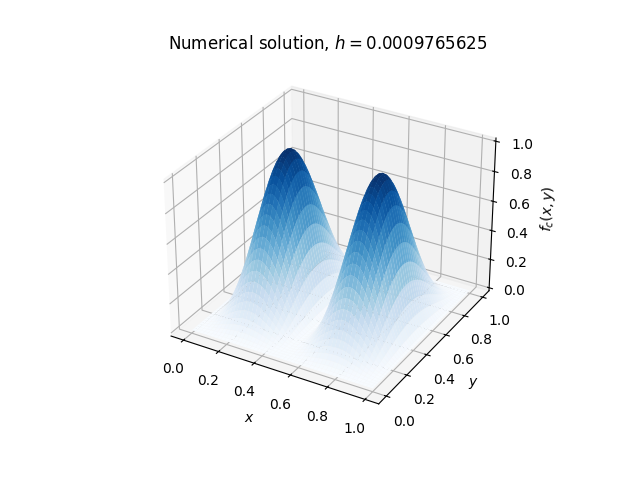
\includegraphics[width=0.65\linewidth]{num_soln.png}
    \caption{Numerical solution, $n=2^{10}$}
    \label{fig:numerical_solution}
\end{figure}

\begin{figure}[h]
    \centering
    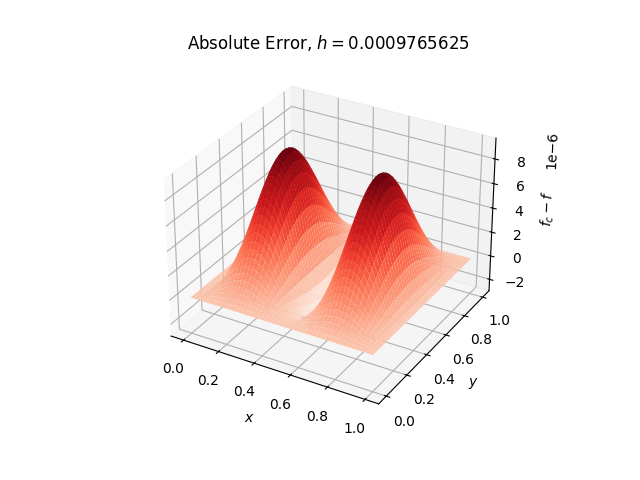
\includegraphics[width=0.65\linewidth]{abs_errs.png}
    \caption{Absolute error, $n=2^{10}$}
    \label{fig:numerical_error}
\end{figure}



% Solutions

\subsection{} 

Scipy's \verb|linalg.onenormest| could be used to estimate the one norm $\norm{\mat{A}}_1$, but does not directly compute the condition number, which requires $\norm{\mat{A}^{-1}}_1$, or an appropriate estimate.

Matlab provides the function \verb|condest|, which uses an iterative method \cite{hager1984condition} that computes the gradient of $f(\vec{x}) = \norm{\mat{A}\vec{x}}_1$, in order to converge on an upper bound for $\norm{\mat{A^{-1}}}_1$. When I tested my own implementation of this algorithm I found its results to be equivalent to directly computing the matrix inverse and using \verb|onenormest|. This iterative estimate appears as \verb|hager_invnorm| in the Python code.

The condition numbers for $n$ up to $2^{10}$ are shown in \autoref{fig:condition}. $\kappa$ shows a clear $\kappa \propto n^{\approx 2}$ increase, clearly justifying the need for a more stable algorithm, potentially different than the GE scheme used in this solve.

\begin{figure}[h]
    \centering
    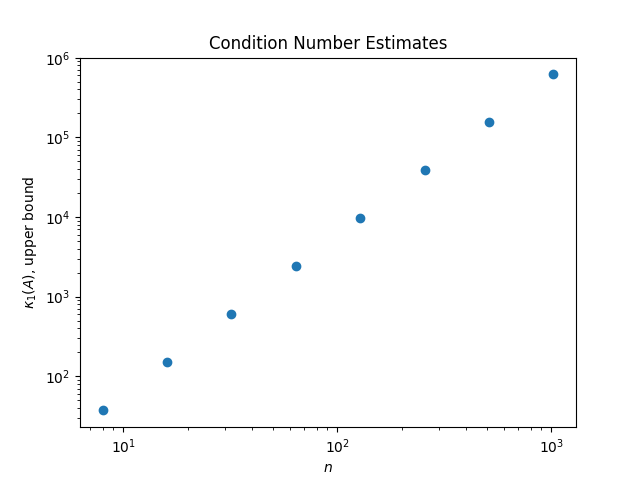
\includegraphics[width=0.65\linewidth]{condition_log.png}
    \caption{Condition number estimates, $\kappa_1(\mat{A})$}
    \label{fig:condition}
\end{figure}


\clearpage

\bibliographystyle{ieeetr}
\bibliography{references}

\appendix

\section{Python Code}\label{sec:code}

\begin{minted}[linenos]{python}
import numpy
# import scipy
import scipy.sparse as sparse
import matplotlib
import matplotlib.pyplot as plt

pi = numpy.pi
# part a -- matrix assignment
def source_function(x, y):
    z = -2*(pi**2)*((numpy.cos(pi*x)**2 * numpy.sin(2*pi*y)**2) 
                    -5*( numpy.sin(pi*x)**2 * numpy.sin(2*pi*y)**2) 
                    +4*(numpy.sin(pi*x)**2 * numpy.cos(2*pi*y)**2))
    return z

def analytic_solution(x, y):
    return numpy.sin(pi*x)**2 * numpy.sin(2*pi*y)**2
    
class poisson_system:
    def __init__(self, x, y, A, f):
        self.x_mesh = x
        self.y_mesh = y
        self.coefficients = A
        self.source = f

def unpack_1d_array(a):
    m = int(numpy.sqrt(a.size))
    n = m+1
    A = numpy.zeros((m,m))
    for i in range(0, m):
        for j in range(0, m):
            A[i][j] = a[i+ (j)*(m)]
    return A

def system_def(f, n):
    m = n-1
    I = sparse.eye(m,m)
    e = numpy.ones(m)
    T = sparse.diags([-e, 4*e, -e], [-1, 0, 1], (m,m))
    S = sparse.diags([-e, -e], [-1, 1], (m,m))
    A = sparse.kron(I, T) + sparse.kron(S, I)
    
    h = 1/n
    x = numpy.arange(h, 1, h)
    y = numpy.arange(h, 1, h)
    q_vec = numpy.zeros((n-1)**2)

    for i in range(0, (n-1)):
        for j in range(0, (n-1)):
            k = i+ (j)*(n-1)
            q_vec[k] = (h**2)*source_function(x[i], y[j])

    return poisson_system(x, y, A, q_vec)

def hager_invnorm(A):
    # Hager 1984, Higham 1988
    n = A.shape[0]
    x = (1/n)*numpy.ones((n))
    while (True):
        y = sparse.linalg.spsolve(A, x)
        # heaviside instead of sign() so that sign(0) = 1
        xi = 2*numpy.heaviside(y, 1) - 1 
        z = sparse.linalg.spsolve(A,xi)
        if (numpy.max(abs(z)) <= z@x):
            return numpy.sum(abs(y))
        x = numpy.zeros(n)
        x[numpy.argmax(z)] = 1


k = numpy.arange(3, 11, 1)
n = 2**k
h = 1/n
e = numpy.zeros(n.shape)
r = e.copy()
cond = e.copy()

for ni in range(0, n.size):
    print("n= "+str(n[ni]))
    system = system_def(source_function, n[ni])
    A = system.coefficients
    x = system.x_mesh
    y = system.y_mesh
    q = system.source

    u = sparse.linalg.spsolve(A, q)
    U = unpack_1d_array(u)
 
    K = numpy.zeros(U.shape)
    for i in range(0, K.shape[0]):
        for j in range(0, K.shape[1]):
            K[i][j] = analytic_solution(x[i], y[j])

    e[ni] = numpy.max(numpy.abs(K-U))
    cond[ni] = sparse.linalg.onenormest(A)*hager_invnorm(A)
    print(cond[ni])
    if (ni>0):
        r[ni] = e[ni]/e[ni-1]
    if n[ni] == 2**10:
        x, y = numpy.meshgrid(x, y)

        fig = plt.figure()
        ax = plt.axes(projection="3d")
        ax.plot_surface(x, y,(U-K), cmap=matplotlib.cm.Reds)
        plt.title("Absolute Error, $h="+str(h[ni])+"$")
        ax.set_xlabel("$x$")
        ax.set_ylabel("$y$")
        ax.set_zlabel("$f_c - f$")
        plt.show()
        # plt.savefig("abs_errs")
        plt.close()

        fig = plt.figure()
        ax = plt.axes(projection="3d")
        ax.plot_surface(x, y,U, cmap=matplotlib.cm.Blues)
        plt.title("Numerical solution, $h="+str(h[ni])+"$")
        ax.set_xlabel("$x$")
        ax.set_ylabel("$y$")
        ax.set_zlabel("$f_c(x,y)$")
        plt.show()
        # plt.savefig("num_soln")
        plt.close()

fig = plt.figure()
plt.scatter(n, cond)
plt.title("Condition Number Estimates")
plt.xlabel("$n$")
plt.ylabel("$\\kappa_1(A)$, upper bound")
plt.show()
# plt.savefig("condition_linear")
plt.xscale("log")
plt.yscale("log")
plt.show()
# plt.savefig("condition_log")
plt.close()

\end{minted}






\end{document}
